%% ODER: format ==         = "\mathrel{==}"
%% ODER: format /=         = "\neq "
%
%
\makeatletter
\@ifundefined{lhs2tex.lhs2tex.sty.read}%
  {\@namedef{lhs2tex.lhs2tex.sty.read}{}%
   \newcommand\SkipToFmtEnd{}%
   \newcommand\EndFmtInput{}%
   \long\def\SkipToFmtEnd#1\EndFmtInput{}%
  }\SkipToFmtEnd

\newcommand\ReadOnlyOnce[1]{\@ifundefined{#1}{\@namedef{#1}{}}\SkipToFmtEnd}
\usepackage{amstext}
\usepackage{amssymb}
\usepackage{stmaryrd}
\DeclareFontFamily{OT1}{cmtex}{}
\DeclareFontShape{OT1}{cmtex}{m}{n}
  {<5><6><7><8>cmtex8
   <9>cmtex9
   <10><10.95><12><14.4><17.28><20.74><24.88>cmtex10}{}
\DeclareFontShape{OT1}{cmtex}{m}{it}
  {<-> ssub * cmtt/m/it}{}
\newcommand{\texfamily}{\fontfamily{cmtex}\selectfont}
\DeclareFontShape{OT1}{cmtt}{bx}{n}
  {<5><6><7><8>cmtt8
   <9>cmbtt9
   <10><10.95><12><14.4><17.28><20.74><24.88>cmbtt10}{}
\DeclareFontShape{OT1}{cmtex}{bx}{n}
  {<-> ssub * cmtt/bx/n}{}
\newcommand{\tex}[1]{\text{\texfamily#1}}	% NEU

\newcommand{\Sp}{\hskip.33334em\relax}


\newcommand{\Conid}[1]{\mathit{#1}}
\newcommand{\Varid}[1]{\mathit{#1}}
\newcommand{\anonymous}{\kern0.06em \vbox{\hrule\@width.5em}}
\newcommand{\plus}{\mathbin{+\!\!\!+}}
\newcommand{\bind}{\mathbin{>\!\!\!>\mkern-6.7mu=}}
\newcommand{\rbind}{\mathbin{=\mkern-6.7mu<\!\!\!<}}% suggested by Neil Mitchell
\newcommand{\sequ}{\mathbin{>\!\!\!>}}
\renewcommand{\leq}{\leqslant}
\renewcommand{\geq}{\geqslant}
\usepackage{polytable}

%mathindent has to be defined
\@ifundefined{mathindent}%
  {\newdimen\mathindent\mathindent\leftmargini}%
  {}%

\def\resethooks{%
  \global\let\SaveRestoreHook\empty
  \global\let\ColumnHook\empty}
\newcommand*{\savecolumns}[1][default]%
  {\g@addto@macro\SaveRestoreHook{\savecolumns[#1]}}
\newcommand*{\restorecolumns}[1][default]%
  {\g@addto@macro\SaveRestoreHook{\restorecolumns[#1]}}
\newcommand*{\aligncolumn}[2]%
  {\g@addto@macro\ColumnHook{\column{#1}{#2}}}

\resethooks

\newcommand{\onelinecommentchars}{\quad-{}- }
\newcommand{\commentbeginchars}{\enskip\{-}
\newcommand{\commentendchars}{-\}\enskip}

\newcommand{\visiblecomments}{%
  \let\onelinecomment=\onelinecommentchars
  \let\commentbegin=\commentbeginchars
  \let\commentend=\commentendchars}

\newcommand{\invisiblecomments}{%
  \let\onelinecomment=\empty
  \let\commentbegin=\empty
  \let\commentend=\empty}

\visiblecomments

\newlength{\blanklineskip}
\setlength{\blanklineskip}{0.66084ex}

\newcommand{\hsindent}[1]{\quad}% default is fixed indentation
\let\hspre\empty
\let\hspost\empty
\newcommand{\NB}{\textbf{NB}}
\newcommand{\Todo}[1]{$\langle$\textbf{To do:}~#1$\rangle$}

\EndFmtInput
\makeatother
%
%
%
%
%
%
% This package provides two environments suitable to take the place
% of hscode, called "plainhscode" and "arrayhscode". 
%
% The plain environment surrounds each code block by vertical space,
% and it uses \abovedisplayskip and \belowdisplayskip to get spacing
% similar to formulas. Note that if these dimensions are changed,
% the spacing around displayed math formulas changes as well.
% All code is indented using \leftskip.
%
% Changed 19.08.2004 to reflect changes in colorcode. Should work with
% CodeGroup.sty.
%
\ReadOnlyOnce{polycode.fmt}%
\makeatletter

\newcommand{\hsnewpar}[1]%
  {{\parskip=0pt\parindent=0pt\par\vskip #1\noindent}}

% can be used, for instance, to redefine the code size, by setting the
% command to \small or something alike
\newcommand{\hscodestyle}{}

% The command \sethscode can be used to switch the code formatting
% behaviour by mapping the hscode environment in the subst directive
% to a new LaTeX environment.

\newcommand{\sethscode}[1]%
  {\expandafter\let\expandafter\hscode\csname #1\endcsname
   \expandafter\let\expandafter\endhscode\csname end#1\endcsname}

% "compatibility" mode restores the non-polycode.fmt layout.

\newenvironment{compathscode}%
  {\par\noindent
   \advance\leftskip\mathindent
   \hscodestyle
   \let\\=\@normalcr
   \let\hspre\(\let\hspost\)%
   \pboxed}%
  {\endpboxed\)%
   \par\noindent
   \ignorespacesafterend}

\newcommand{\compaths}{\sethscode{compathscode}}

% "plain" mode is the proposed default.
% It should now work with \centering.
% This required some changes. The old version
% is still available for reference as oldplainhscode.

\newenvironment{plainhscode}%
  {\hsnewpar\abovedisplayskip
   \advance\leftskip\mathindent
   \hscodestyle
   \let\hspre\(\let\hspost\)%
   \pboxed}%
  {\endpboxed%
   \hsnewpar\belowdisplayskip
   \ignorespacesafterend}

\newenvironment{oldplainhscode}%
  {\hsnewpar\abovedisplayskip
   \advance\leftskip\mathindent
   \hscodestyle
   \let\\=\@normalcr
   \(\pboxed}%
  {\endpboxed\)%
   \hsnewpar\belowdisplayskip
   \ignorespacesafterend}

% Here, we make plainhscode the default environment.

\newcommand{\plainhs}{\sethscode{plainhscode}}
\newcommand{\oldplainhs}{\sethscode{oldplainhscode}}
\plainhs

% The arrayhscode is like plain, but makes use of polytable's
% parray environment which disallows page breaks in code blocks.

\newenvironment{arrayhscode}%
  {\hsnewpar\abovedisplayskip
   \advance\leftskip\mathindent
   \hscodestyle
   \let\\=\@normalcr
   \(\parray}%
  {\endparray\)%
   \hsnewpar\belowdisplayskip
   \ignorespacesafterend}

\newcommand{\arrayhs}{\sethscode{arrayhscode}}

% The mathhscode environment also makes use of polytable's parray 
% environment. It is supposed to be used only inside math mode 
% (I used it to typeset the type rules in my thesis).

\newenvironment{mathhscode}%
  {\parray}{\endparray}

\newcommand{\mathhs}{\sethscode{mathhscode}}

% texths is similar to mathhs, but works in text mode.

\newenvironment{texthscode}%
  {\(\parray}{\endparray\)}

\newcommand{\texths}{\sethscode{texthscode}}

% The framed environment places code in a framed box.

\def\codeframewidth{\arrayrulewidth}
\RequirePackage{calc}

\newenvironment{framedhscode}%
  {\parskip=\abovedisplayskip\par\noindent
   \hscodestyle
   \arrayrulewidth=\codeframewidth
   \tabular{@{}|p{\linewidth-2\arraycolsep-2\arrayrulewidth-2pt}|@{}}%
   \hline\framedhslinecorrect\\{-1.5ex}%
   \let\endoflinesave=\\
   \let\\=\@normalcr
   \(\pboxed}%
  {\endpboxed\)%
   \framedhslinecorrect\endoflinesave{.5ex}\hline
   \endtabular
   \parskip=\belowdisplayskip\par\noindent
   \ignorespacesafterend}

\newcommand{\framedhslinecorrect}[2]%
  {#1[#2]}

\newcommand{\framedhs}{\sethscode{framedhscode}}

% The inlinehscode environment is an experimental environment
% that can be used to typeset displayed code inline.

\newenvironment{inlinehscode}%
  {\(\def\column##1##2{}%
   \let\>\undefined\let\<\undefined\let\\\undefined
   \newcommand\>[1][]{}\newcommand\<[1][]{}\newcommand\\[1][]{}%
   \def\fromto##1##2##3{##3}%
   \def\nextline{}}{\) }%

\newcommand{\inlinehs}{\sethscode{inlinehscode}}

% The joincode environment is a separate environment that
% can be used to surround and thereby connect multiple code
% blocks.

\newenvironment{joincode}%
  {\let\orighscode=\hscode
   \let\origendhscode=\endhscode
   \def\endhscode{\def\hscode{\endgroup\def\@currenvir{hscode}\\}\begingroup}
   %\let\SaveRestoreHook=\empty
   %\let\ColumnHook=\empty
   %\let\resethooks=\empty
   \orighscode\def\hscode{\endgroup\def\@currenvir{hscode}}}%
  {\origendhscode
   \global\let\hscode=\orighscode
   \global\let\endhscode=\origendhscode}%

\makeatother
\EndFmtInput
%
%
%
% First, let's redefine the forall, and the dot.
%
%
% This is made in such a way that after a forall, the next
% dot will be printed as a period, otherwise the formatting
% of `comp_` is used. By redefining `comp_`, as suitable
% composition operator can be chosen. Similarly, period_
% is used for the period.
%
\ReadOnlyOnce{forall.fmt}%
\makeatletter

% The HaskellResetHook is a list to which things can
% be added that reset the Haskell state to the beginning.
% This is to recover from states where the hacked intelligence
% is not sufficient.

\let\HaskellResetHook\empty
\newcommand*{\AtHaskellReset}[1]{%
  \g@addto@macro\HaskellResetHook{#1}}
\newcommand*{\HaskellReset}{\HaskellResetHook}

\global\let\hsforallread\empty

\newcommand\hsforall{\global\let\hsdot=\hsperiodonce}
\newcommand*\hsperiodonce[2]{#2\global\let\hsdot=\hscompose}
\newcommand*\hscompose[2]{#1}

\AtHaskellReset{\global\let\hsdot=\hscompose}

% In the beginning, we should reset Haskell once.
\HaskellReset

\makeatother
\EndFmtInput
















%%format ._ = "."








% format runC         = "run\mathbb{C}_{\scalebox{0.6}{T}}"
% format C            = "\mathbb{C}_{\scalebox{0.6}{T}}"
%%format R            = "\mathbb{R}_{\scalebox{0.6}{T}}"



\begin{figure}[t!]
  \fbox{
  \begin{minipage}{.95\columnwidth}
     \hspace{-1.5cm}\begin{minipage}{1.15\columnwidth}
      \infrule[WFM-Illtyped]{}{
        \Sigma \vdash_M \ensuremath{\Varid{v}_\Varid{m}} ~:~ \ensuremath{\Varid{fail}}
      }
      \vspace{.25cm}
      \hspace{-1cm} \infrule[WFM-Return] {
         \Sigma \vdash v ~:~ t
      }
      {
       \Sigma \vdash_M \ensuremath{\Varid{return}\;\Varid{v}} ~:~ \ensuremath{\Varid{return}\;\Varid{t}}
      }
  \end{minipage}
  \end{minipage}
 }
\caption{Typing rules for pure monadic values.}
\label{fig:WFM+Pure}
\vspace{-.4cm}
\end{figure}

\section{Modular Monadic Type Soundness}


In order to preserve a measure of modularity, we do not prove type
soundness directly for a given feature, but by means of a more generic
theorem. The technique of proving a theorem of interest by means of a
more general theorem is well-known. For a conventional monolithic
language, for instance, type soundness is often established for any
well-formed typing context, even though the main interest lies with
the more specific initial, empty context. In that setting, the more
general theorem produces a weaker induction hypothesis for the
theorem's proof.

Our approach to type soundness follows the core idea of this technique
and relies on three theorems:

{\addtolength{\leftskip}{5mm}
\noindent \hspace{-.25cm} \textsc{FSound}:
 a reusable \emph{feature theorem} that is only aware of the effects that
 a feature uses \par}

{\addtolength{\leftskip}{5mm}
\noindent \hspace{-.25cm} \textsc{ESound}:
 an \emph{effect theorem} for a fixed set of known effects, and \par}

{\addtolength{\leftskip}{5mm}
\noindent\hspace{-.25cm} \textsc{LSound}: a \emph{language theorem} which combines the two
to prove soundness for a specific language.
\par }

\noindent In order to maximize compatibility, the statement of the
reusable feature theorem cannot hardwire the set of effects. This
statement must instead rephrase type soundness in a way that can adapt
to any superset of a feature's effects. Our solution is to have the
feature theorem establish that the monadic evaluation and typing
algebras of a feature satisfy an extensible well-formedness relation,
defined in terms of effect-specific typing rules. Thus, a
feature's proof of \ref{thm:FSound} uses only the typing rules required
for the effects specific to that feature. The final language combines
the typing rules of all the language's effects into a closed relation.

\begin{figure}[t!]
  \fbox{
  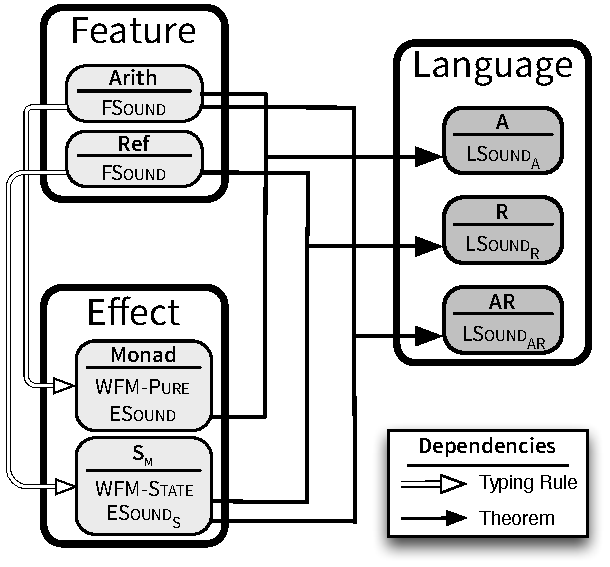
\includegraphics[scale = .77]{src/ModularEffects/Dependency-1.pdf}
   }
\caption{Dependency Graph}
\label{fig:Dep-Graph}
\end{figure}

Figure~\ref{fig:Dep-Graph} illustrates how these reusable pieces fit
together to build a proof of soundness. Each feature provides a proof
algebra for \ref{thm:FSound} which relies on the typing rules
(\textsc{WFM-X}) for the effects it uses. Each unique statement of
soundness for a combination of effects requires a new proof of
\textsc{ESound}. The proof of \ref{thm:LSoundP} for a particular
language is synthesized entirely from a single proof of
\textsc{ESound} and a combination of proof algebras for
\ref{thm:FSound}.

Note that there are several dimensions of modularity here. A feature's
proof of \ref{thm:FSound} only depends on the typing rules for the
effects that feature uses and can thus be used in any language which
includes those typing rules. The typing rules themselves can be reused
by any number of different features. \textsc{ESound} depends solely on
a specific combination of effects and can be reused in any language
which supports that unique combination, e.g. both
\textsc{LSound$_{A}$} and \textsc{LSound$_{AR}$} use
\textsc{ESound$_{ES}$}.


% around an extensible relation, which relates two
% monadic computations.
% To acheive extensibility, we prove that an extensible
% relation holds over the monadic values of the evaluation function and
% the typing function of each language feature. Each effect will have
% its own set of typing rules used by each feature which uses that
% effect. The final relation is the composition of the typing rules for
% the set of effects in the final language.

% An important modularity property of the typing rules is that they only
% depend on the effects and not on the features. This enables us to
% decouple the proof that a feature's semantics obeys the extensible
% relation from the proof that the closed relation entails the actual
% property of interest, type soundness. The latter proof does
% not depend on the particular features involved, only on the
% effects. The rules reflect the other dimension of modularity: we can now
% have effect modules which are independent of language features
% (although the latter depend on the former). Thus, soundness theorems
% need to be proven only once for each combination of effects, and can
% be reused for any language with that combination of effects.

% Figures~\ref{fig:WFM+Pure}-\ref{fig:WFM+Except} provide examples of
% the judgements of this monadic well-formedness relation. In essence,
% each rule defines how to type a monadic value which binds an operation
% of that monad. Each effect-specific soundness proof proceeds by
% induction on this relation; in each case showing how to 'process' this
% function according to the specific set of effects and then using the
% inductive hypothesis for the computation resulting from binding the
% result.

%-------------------------------------------------------------------------------
\subsection{Soundness for a Pure Feature}

%- - - - - - - - - - - - - - - - - - - - - - - - - - - - - - - - - - - - - - - -
\label{sec:Thm+Reuse}

The reusable feature theorem \ref{thm:FSound} states that \ensuremath{\llbracket \cdot \rrbracket} and
\ensuremath{\Varid{typeof}} are related by the extensible typing relation:
\begin{equation}
  \forall e, \Sigma.\quad\Sigma \vdash_M \ensuremath{\llbracket \Varid{e}\rrbracket} : \ensuremath{\Varid{typeof}\;\Varid{e}}
\tag{\textsc{FSound}}
\label{thm:FSound}
\end{equation}

\paragraph{Extensible Typing Relation} The extensible
typing relation has the form: \[ \Sigma \vdash_M v_m : t_m \] The
relation is polymorphic in an environment type \ensuremath{\Varid{env}} and an evaluation
monad type \ensuremath{\Varid{m}}.  The parameters $\Sigma$, $v_m$ and $t_m$ have types
\ensuremath{\Varid{env}}, \ensuremath{\Varid{m}\;\Conid{Value}} and \ensuremath{\Conid{Maybe}\;\Conid{Type}} respectively.
% \BO{using |m_e| and
%|m_t| may be confused with the monad type |m|.  Maybe some different
%variable names are better? (This is low priority: if there's time,
%because we need to make sure everything is consistently patched)}.
The modular typing rules for this relation can impose constraints on
the environment type \ensuremath{\Varid{env}} and monad type \ensuremath{\Varid{m}}. A particular language must
instantiate \ensuremath{\Varid{env}} and \ensuremath{\Varid{m}} in a way that satisfies all the
constraints imposed by the typing rules used in its features.

Figure~\ref{fig:WFM+Pure} lists the two base typing rules of this
relation. These do not constrain the evaluation monad and environment
types and are the only rules needed for pure features. The
\textsc{(WFM-Illtyped)} rule denotes that nothing can be
said about computations (\ensuremath{\Varid{m}_\Varid{e}}) which are ill-typed.
The \textsc{(WFM-Return)} rule ensures that well-typed computations only
yield values of the expected type.

To see how the reusable theorem works for a pure feature, consider the proof
of soundness for the boolean feature.


\paragraph{Proof} Using the above two rules, we can show that
\ref{thm:FSound} holds for the boolean feature. The proof
has two cases.  The boolean literal case is handled by a
trivial application of \textsc{(WFM-Return)}. The second case, for
conditionals, is more interesting\footnote{We omit the environment $\Sigma$ to avoid clutter.}.
\vspace{-1mm}
\begin{multline*}
(\vdash_M \ensuremath{\llbracket \Varid{e\char95 c}\rrbracket}~:~\ensuremath{\Varid{typeof}\;\Varid{e\char95 c}}) \rightarrow \\
\hspace{-2cm}(\vdash_M \ensuremath{\llbracket \Varid{e\char95 t}\rrbracket}~:~\ensuremath{\Varid{typeof}\;\Varid{e\char95 t}}) \rightarrow \\
   (\vdash_M \ensuremath{\llbracket \Varid{e\char95 e}\rrbracket}~:~\ensuremath{\Varid{typeof}\;\Varid{e\char95 e}}) \rightarrow \\
 \vdash_M \left(\hspace{-5mm}
\begin{minipage}{37mm}
\begin{hscode}\SaveRestoreHook
\column{B}{@{}>{\hspre}l<{\hspost}@{}}%
\column{3}{@{}>{\hspre}l<{\hspost}@{}}%
\column{7}{@{}>{\hspre}l<{\hspost}@{}}%
\column{10}{@{}>{\hspre}l<{\hspost}@{}}%
\column{12}{@{}>{\hspre}l<{\hspost}@{}}%
\column{18}{@{}>{\hspre}l<{\hspost}@{}}%
\column{19}{@{}>{\hspre}l<{\hspost}@{}}%
\column{E}{@{}>{\hspre}l<{\hspost}@{}}%
\>[3]{}\mathbf{do}\;{}\<[7]%
\>[7]{}\Varid{v}\leftarrow \llbracket \Varid{e\char95 c}\rrbracket{}\<[E]%
\\
\>[7]{}\mathbf{case}\;\Varid{isBool}\;\Varid{v}\;\mathbf{of}{}\<[E]%
\\
\>[7]{}\hsindent{3}{}\<[10]%
\>[10]{}\Conid{Just}\;\Varid{b}{}\<[19]%
\>[19]{}\to {}\<[E]%
\\
\>[10]{}\hsindent{2}{}\<[12]%
\>[12]{}\mathbf{if}\;\Varid{b}\;{}\<[18]%
\>[18]{}\mathbf{then}\;\llbracket \Varid{e\char95 t}\rrbracket{}\<[E]%
\\
\>[18]{}\mathbf{else}\;\llbracket \Varid{e\char95 e}\rrbracket{}\<[E]%
\\
\>[7]{}\hsindent{3}{}\<[10]%
\>[10]{}\Conid{Nothing}{}\<[19]%
\>[19]{}\to \Varid{stuck}{}\<[E]%
\ColumnHook
\end{hscode}\resethooks
\end{minipage}
\right) :
\left(\hspace{-5mm}
\begin{minipage}{35mm}
\begin{hscode}\SaveRestoreHook
\column{B}{@{}>{\hspre}l<{\hspost}@{}}%
\column{3}{@{}>{\hspre}l<{\hspost}@{}}%
\column{7}{@{}>{\hspre}l<{\hspost}@{}}%
\column{E}{@{}>{\hspre}l<{\hspost}@{}}%
\>[3]{}\mathbf{do}\;{}\<[7]%
\>[7]{}\Varid{t}_\Varid{c}\leftarrow \Varid{typeof}\;\Varid{e\char95 c}{}\<[E]%
\\
\>[7]{}\Varid{t}_\Varid{t}\leftarrow \Varid{typeof}\;\Varid{e\char95 t}{}\<[E]%
\\
\>[7]{}\Varid{t}_\Varid{e}\leftarrow \Varid{typeof}\;\Varid{e\char95 e}{}\<[E]%
\\
\>[7]{}\Varid{guard}\;(\Varid{isTBool}\;\Varid{t}_\Varid{c}){}\<[E]%
\\
\>[7]{}\Varid{guard}\;(\Varid{eqT}\;\Varid{t}_\Varid{t}\;\Varid{t}_\Varid{e}){}\<[E]%
\\
\>[7]{}\Varid{return}\;\Varid{t}_\Varid{t}{}\<[E]%
\ColumnHook
\end{hscode}\resethooks
\end{minipage}
\right)
\tag{\textsc{WFM-If-Vc}}
\label{thm:WFM+If+Vc}
\end{multline*}
\vspace{-2mm}
% \BO{Another comment. Earlier we talk about the monad |m| (lowercase), here we use
% the subscript |M| (uppercase). Should these be the same?}

% TOM: I think we don't have to talk about lockstep here because we don't
%      mention it before either. It would only be distracting and confusing
%      to cover a failed attempt at tackling monads.
%
% The proof algebra that $\vdash_M$
% |(eval e) : typeof e| has a case for boolean literals and another for
% conditionals. The goal in the second case simplifies to $\vdash_M$ |(do
% v_c <- eval c; ...) : do T_c <- typeof; ... |. \BD{Latex this formula
% correctly.}  Observe there is a disconnect between the monadic values
% returned by the two functions. This is a common occurence, as |eval|
% can dynamically decide which subexpressions to evaluate while |typeof|
% must consider every subexpression in order to be a proper static
% semantic function. The desire to have a more flexible relation
% (i.e. not lockstep) motivates the formulation of \textsc{WFM-Return}
% in Fig.~\ref{fig:WFM+Pure}.

Because \ensuremath{\llbracket \cdot \rrbracket} and \ensuremath{\Varid{typeof}} are polymorphic in the monad, we cannot
directly inspect the values they produce. We can, however, perform
case analysis on the derivations of the proofs produced by the
induction hypothesis that the subexpressions are well-formed,
$\vdash_M$~\ensuremath{\llbracket \Varid{e\char95 c}\rrbracket}~:~\ensuremath{\Varid{typeof}\;\Varid{e\char95 c}},
$\vdash_M$~\ensuremath{\llbracket \Varid{e\char95 t}\rrbracket}~:~\ensuremath{\Varid{typeof}\;\Varid{e\char95 t}}, and
$\vdash_M$~\ensuremath{\llbracket \Varid{e\char95 e}\rrbracket}~:~\ensuremath{\Varid{typeof}\;\Varid{e\char95 e}}. The final rule used in each derivation determines the shape of
the monadic value produced by \ensuremath{\llbracket \cdot \rrbracket} and \ensuremath{\Varid{typeof}}.
Assuming that only the pure typing rules of Figure~\ref{fig:WFM+Pure}
are used for the derivations, we can divide the proof into
two cases depending on whether \ensuremath{\Varid{e\char95 c}}, \ensuremath{\Varid{e\char95 t}}, or \ensuremath{\Varid{e\char95 e}} was typed with \textsc{(WFM-Illtyped)}.
\begin{itemize}
\item
If any of the three derivations uses \textsc{(WFM-Illtyped)},
the result of \ensuremath{\Varid{typeof}} is \ensuremath{\Varid{fail}}. As \ensuremath{\Varid{fail}} is the zero of the typing
monad, \textsc{(WFM-Illtyped)} resolves the case.
\item
Otherwise, each of the subderivations was built with
\textsc{(WFM-Return)} and the evaluation and typing expressions can
be simplified using the \ensuremath{\Varid{return\char95 bind}} monad law.
\[ \hspace{-5mm}\vdash_M \left(\hspace{-5mm}
\begin{minipage}{37mm}
\begin{hscode}\SaveRestoreHook
\column{B}{@{}>{\hspre}l<{\hspost}@{}}%
\column{3}{@{}>{\hspre}l<{\hspost}@{}}%
\column{6}{@{}>{\hspre}l<{\hspost}@{}}%
\column{8}{@{}>{\hspre}l<{\hspost}@{}}%
\column{14}{@{}>{\hspre}l<{\hspost}@{}}%
\column{15}{@{}>{\hspre}l<{\hspost}@{}}%
\column{E}{@{}>{\hspre}l<{\hspost}@{}}%
\>[3]{}\mathbf{case}\;\Varid{isBool}\;\Varid{v}_\Varid{c}\;\mathbf{of}{}\<[E]%
\\
\>[3]{}\hsindent{3}{}\<[6]%
\>[6]{}\Conid{Just}\;\Varid{b}{}\<[15]%
\>[15]{}\to {}\<[E]%
\\
\>[6]{}\hsindent{2}{}\<[8]%
\>[8]{}\mathbf{if}\;\Varid{b}\;{}\<[14]%
\>[14]{}\mathbf{then}\;\Varid{return}\;\Varid{v}_\Varid{t}{}\<[E]%
\\
\>[14]{}\mathbf{else}\;\Varid{return}\;\Varid{v}_\Varid{e}{}\<[E]%
\\
\>[3]{}\hsindent{3}{}\<[6]%
\>[6]{}\Conid{Nothing}{}\<[15]%
\>[15]{}\to \Varid{stuck}{}\<[E]%
\ColumnHook
\end{hscode}\resethooks
\end{minipage}
\right) :
\left(\hspace{-5mm}
\begin{minipage}{35mm}
\begin{hscode}\SaveRestoreHook
\column{B}{@{}>{\hspre}l<{\hspost}@{}}%
\column{3}{@{}>{\hspre}l<{\hspost}@{}}%
\column{7}{@{}>{\hspre}l<{\hspost}@{}}%
\column{E}{@{}>{\hspre}l<{\hspost}@{}}%
\>[3]{}\mathbf{do}\;{}\<[7]%
\>[7]{}\Varid{guard}\;(\Varid{isTBool}\;\Varid{t}_\Varid{c}){}\<[E]%
\\
\>[7]{}\Varid{guard}\;(\Varid{eqT}\;\Varid{t}_\Varid{t}\;\Varid{t}_\Varid{e}){}\<[E]%
\\
\>[7]{}\Varid{return}\;\Varid{t}_\Varid{t}{}\<[E]%
\ColumnHook
\end{hscode}\resethooks
\end{minipage}
\right)
\]
After simplification, the typing expression has replaced the bind with
explicit values which can be reasoned with. If \ensuremath{\Varid{isTBool}\;\Varid{t}_\Varid{c}} is \ensuremath{\Varid{false}}, then
the typing expression reduces to \ensuremath{\Varid{fail}} and well-formedness again follows from the
\textsc{WFM-Illtyped} rule. Otherwise \ensuremath{\Varid{t}_\Varid{c}\equiv \Conid{TBool}}, and we
can apply the inversion lemma
\[ \vdash \ensuremath{\Varid{v}} : \ensuremath{\Conid{TBool}} \rightarrow \exists b. \ensuremath{\Varid{isBool}\;\Varid{v}\equiv \Conid{Just}\;\Varid{b}} \] to
establish that \ensuremath{\Varid{v}_\Varid{c}} is of the form \ensuremath{\Conid{Just}\;\Varid{b}}, reducing the evaluation
to either \ensuremath{\Varid{return}\;\Varid{v}_\Varid{e}} or \ensuremath{\Varid{return}\;\Varid{v}_\Varid{t}}. A similar case analysis on
\ensuremath{\Varid{eqT}\;\Varid{t}_\Varid{t}\;\Varid{t}_\Varid{e}} will either produce \ensuremath{\Varid{fail}} or \ensuremath{\Varid{return}\;\Varid{t}_\Varid{t}}. The former
is trivially true, and both $\vdash_M \ensuremath{\Varid{return}\;\Varid{v}_\Varid{t}}:\ensuremath{\Varid{return}\;\Varid{t}_\Varid{t}}$ and $\vdash_M \ensuremath{\Varid{return}\;\Varid{v}_\Varid{e}}:\ensuremath{\Varid{return}\;\Varid{t}_\Varid{t}}$ hold
in the latter case from the induction hypotheses.
%
% \tom{Need more clarification here.}
% In
% the \textsc{WFM-Return} case, |(do v_c <- eval c; ...)| simplifies to
% either |Stuck|, |eval t|, or |eval e|. In the first case, we can push
% the type information in the refinement type of |T_c'| from the
% \textsc{WFM-Return} rule used to build the current case into the body
% of the bind expression to ensure that |do T_c <- typeof c; ...| will
% evaluate to |fail|, from which \textsc{WFM-Untyped} applies. The
% refinement type of the |T_c'| monad can be used analogously in the
% other two cases to ensure that |typeof c| always produces |TBool|, and
% \textsc{WFM-Return} can then be applied.
\end{itemize}

\paragraph{Modular Sublemmas} The above proof assumed that only the
pure typing rules of Figure~\ref{fig:WFM+Pure} were used to type the
subexpressions of the \ensuremath{\mathbf{if}} expression, which is clearly not the case
when the boolean feature is included in an effectful
language. Instead, case analyses are performed on the extensible
typing relation in order to make the boolean feature theorem
compatible with new effects. Case analyses over the extensible
$\vdash_M$ relation are accomplished using extensible proof algebras
which are folded over the derivations provided by the induction
hypothesis, as outlined in Section~\ref{subsec:modproofs}.

In order for the boolean feature's proof of \ref{thm:FSound} to be
compatible with a new effect, each extensible case analysis requires a
proof algebra for the new typing rules the effect introduces to the $\vdash_M$
relation. These proof algebras are examples of
\emph{feature interactions}~\cite{featureinteractions} from the
setting of modular component-based frameworks. In essence, a feature
interaction is functionality (e.g., a function or a proof) that is
only necessary when two features are combined. Importantly, these
proof algebras do not need to be provided up front when developing the
boolean algebra, but can instead be modularly resolved by a separate
feature for the interaction of booleans and the new effect.



The formulation of the properties proved by extensible case analysis
has an impact on modularity. The conditional case of the previous
proof can be dispatched by folding a proof algebra for the property
\ref{thm:WFM+If+Vc} over $\vdash_M~\ensuremath{\llbracket \Varid{v}_\Varid{c}\rrbracket}~:~\ensuremath{\Varid{typeof}\;\Varid{t}_\Varid{c}}$. Each
new effect induces a new case for this proof algebra, however,
resulting in an interaction between booleans and every
effect. \ref{thm:WFM+If+Vc} is specific to the proof of
\ref{thm:FSound} in the boolean feature; proofs of \ref{thm:FSound}
for other features require different properties and thus different
proof algebras. Relying on such specific properties can lead to a
proliferation of proof obligations for each new effect.

Alternatively, the boolean feature can use a proof algebra for a
stronger property that is also applicable in other proofs, cutting
down on the number of feature interactions. One such stronger, more
general sublemma relates the monadic bind operation to well-typing:
\begin{multline}
 (\Sigma\vdash_M~~ v_m ~:~t_m) \rightarrow \\
   (\forall v~T~\Sigma'\supseteq\Sigma.~(\Sigma'\vdash~v~:~T) \rightarrow
   ~\Sigma'\vdash_M~~ k_v~v~:~ k_t~T) \rightarrow \\
   \Sigma\vdash_M~~v_m \ensuremath{\bind } k_v~:~t_m \ensuremath{\bind } k_t
\tag{\textsc{WFM-Bind}}\label{thm:WFM+Bind}
\end{multline}

A proof of \textsc{WFM-If-Vc} follows from two applications of this
stronger property. The advantage of \textsc{WFM-Bind} is clear: it can
be reused to deal with case analyses in other proofs of
\ref{thm:FSound}, while a proof of \ref{thm:WFM+If+Vc} has only a
single use. The disadvantage is that \textsc{WFM-Bind} may not hold
for some new effect, while the weaker \ref{thm:WFM+If+Vc} does,
possibly excluding some feature combinations. As \textsc{WFM-Bind} is
a desirable property for typing rules, the case study focuses on that
approach.

% \BD{Maybe we
%should expound on this in the case study section- Lambda uses
%WFM-Bind to cut down on feature interactions. }


%- - - - - - - - - - - - - - - - - - - - - - - - - - - - - - - - - - - - - - - -
\subsection{Type Soundness for a Pure Language}

The second phase of showing type soundness is to prove a statement of
soundness for a fixed set of effects. For pure effects, the
soundness statement is straightforward:
\begin{equation}
\forall \ensuremath{\Varid{v}_\Varid{m}}~\ensuremath{\Varid{t}}. \vdash_M \ensuremath{\Varid{v}_\Varid{m}\mathbin{:}\Varid{return}\;\Varid{t}} \Rightarrow \exists \ensuremath{\Varid{v}}. \ensuremath{\Varid{v}_\Varid{m}\equiv \Varid{return}\;\Varid{v}}~\wedge \vdash \ensuremath{\Varid{v}} : \ensuremath{\Varid{t}}
\tag{\textsc{ESound}$_P$}\label{thm:ESoundP}
\end{equation}

Each effect theorem is proved by induction over the derivation of
$\vdash_M$ \ensuremath{\Varid{v}_\Varid{m}\mathbin{:}\Varid{return}\;\Varid{t}}. \ref{thm:ESoundP} fixes the
irrelevant environment type to the type \ensuremath{()} and the evaluation monad
to the pure monad \ensuremath{\mathbb{I}}. Since the evaluation monad is fixed, the proof
of \ref{thm:ESoundP} only needs to consider the pure typing rules of
Figure~\ref{fig:WFM+Pure}. The proof of the effect theorem is
straightforward: \textsc{WFM-Illtyped} could not have been used to derive
$\vdash_M \ensuremath{\Varid{v}_\Varid{m}\mathbin{:}\Varid{return}\;\Varid{t}}$, and \textsc{WFM-Return} provides both a witness
for \ensuremath{\Varid{v}} and a proof that it is of type \ensuremath{\Varid{t}}.

The statement of soundness for a pure language built from a particular
set of features is similar to \ref{thm:ESoundP}:
\begin{equation}
\forall \ensuremath{\Varid{e}}, \ensuremath{\Varid{t}}. \ensuremath{\Varid{typeof}\;\Varid{e}\equiv \Varid{return}\;\Varid{t}} \Rightarrow \exists \ensuremath{\Varid{v}}. \ensuremath{\llbracket \Varid{e}\rrbracket\equiv \Varid{return}\;\Varid{v}}~\wedge \vdash \ensuremath{\Varid{v}} : \ensuremath{\Varid{t}}
\tag{\textsc{LSound}}\label{thm:LSoundP}
\end{equation}

The proof of \ref{thm:LSoundP} is an immediate consequence of the
reusable proofs of \ref{thm:FSound} and \ref{thm:ESoundP}. Folding a
proof algebra for \ref{thm:FSound} over \ensuremath{\Varid{e}} provides a proof of
$\vdash_M \ensuremath{\llbracket \Varid{e}\rrbracket\mathbin{:}\Varid{return}\;\Varid{t}}$, satisfying the first assumption of
\ref{thm:ESoundP}.  \ref{thm:LSoundP} follows immediately.

%Since this proof of \ref{thm:FSound} only depends on the typing rules
%used and not on the particular features involved, it can be reused for
%any other pure language, e.g. any combination of booleans and
%arithmetic expressions. Proofs of type soundness for a particular set
%of effects are similarly divorced from a language's features,
%depending only on the set of typing rules (and thus effects) included
%in a language.

%The proof proceeds by straightforward case analysis of the typing rules of Fig.~\ref{fig:WFM+Pure}.
% \tom{This text does not yet assume that the typing monad is fixed:}
% \begin{itemize}
% \item
% The
% case for \textsc{WFM-Return} depends on another property of the |MT|
% monad used in the |typeof| function:
%
% < forall A B (ma :: M A) (f :: A -> B) b,
% <    fmap f ma = return b -> exists a._ f a = b
%
% This allows us to 'lift' a proof out of any monad with refinement type
% whose proof component has been projected out. This allows us to
% conclude that all the types in |typeof e| equal |t|, and soundness
% follows immediately from the assumptions of
% \textsc{WFM-Return}.
% \item
% Furthermore, a corollary of this law is that
% |forall v._ fail <> return v|, which in the \textsc{WFM-Untyped} case
% contradicts the assumption that |typeof e = return t|. The latter case
% demonstrates the important point that the set of effects is fixed in
% the specialized soundness theorems, allowing the proof to reason about
% the complete set of operations. In the pure case, for example, the
% proof can safely assume that |typeof e| will either equal |fail| or
% there will exists some |T| such that |typeof e = return T|. This will
% be useful in the next section.
% \end{itemize}
%
%
%Note however that the typing rules are independent of the particular feature
%used; they only depend on the effect. This means that the same specific proof can be
%reused for all pure features as long as they supply a proof algebra for the
%pure typing rules.



%-------------------------------------------------------------------------------

\begin{figure}
  \fbox{
  \begin{minipage}{.95\columnwidth}
     \hspace{-2.1cm}\begin{minipage}{1.25\columnwidth}
      \infrule[WFM-Throw]{
      }
      {
        \Sigma \vdash_M \ensuremath{\Varid{throw}\;\Varid{x}} ~:~ \ensuremath{\Varid{t}_\Varid{m}}
      }
    \vspace{.25cm}
      \infrule[WFM-Catch]
      {
        \Sigma \vdash_M \ensuremath{\Varid{m}\bind \Varid{k}}  ~:~ \ensuremath{\Varid{t}_\Varid{m}} \\
        \forall~\Sigma' \supseteq \Sigma~\ensuremath{\Varid{x}}~.~\Sigma' \vdash_M \ensuremath{\Varid{h}\;\Varid{x}\bind \Varid{k}} ~:~ \ensuremath{\Varid{t}_\Varid{m}}
      }
      {
         \Sigma \vdash_M \ensuremath{\Varid{catch}\;\Varid{m}\;\Varid{h}\bind \Varid{k}} ~:~ \ensuremath{\Varid{t}_\Varid{m}}
      }
  \end{minipage}
  \end{minipage}
 }
\caption{Typing rules for exceptional monadic values.}
\label{fig:WFM+Except}
\vspace{-.4cm}
\end{figure}

%-------------------------------------------------------------------------------
\subsection{Errors}

The evaluation algebra of the error language feature uses the side
effects of the exception monad, requiring new typing rules.

\paragraph{Typing Rules}

Figure~\ref{fig:WFM+Except} lists the typing rules for monadic
computations involving exceptions. \textsc{WFM-Throw} states that
\ensuremath{\Varid{throw}\;\Varid{x}} is typeable with any type. \textsc{WFM-Catch} states that
binding the results of both branches of a \ensuremath{\Varid{catch}} statement will
produce a monad with the same type. While it may seem odd that this
rule is formulated in terms of a continuation \ensuremath{\bind \Varid{k}}, it is essential
for compatibility with the proofs algebras required by other
features. As described in Section~\ref{sec:Thm+Reuse}, extensible
proof algebras over the typing derivation will now need cases for the
two new rules. To illustrate this, consider the proof algebra for the
general purpose \ref{thm:WFM+Bind} property. This algebra requires a
proof of:
\begin{multline*}
 (\Sigma\vdash_M\ensuremath{\Varid{catch}\;\Varid{e}\;\Varid{h}\bind \Varid{k}} ~:~t_m) \rightarrow \\
   (\forall v~T~\Sigma'\supseteq\Sigma.~(\Sigma'\vdash~v~:~T) \rightarrow
   ~\Sigma'\vdash_M~~ k_v~v~:~ k_t~T) \rightarrow \\
   \Sigma\vdash_M(\ensuremath{\Varid{catch}\;\Varid{e}\;\Varid{h}\bind \Varid{k}}) \ensuremath{\bind } k_v:t_m \ensuremath{\bind } k_t
\end{multline*}


With the continuation, we can first apply the associativity law to
reorder the binds so that \textsc{WFM-Catch} can be applied: \ensuremath{(\Varid{catch}\;\Varid{e}\;\Varid{h}\bind \Varid{k})\bind } $k_v$ \ensuremath{\mathrel{=}\Varid{catch}\;\Varid{e}\;\Varid{h}\bind (\Varid{k}\bind }$k_v)$. The two premises
of the rule follow immediately from the inductive hypothesis of the
lemma, finishing the proof. Without the continuation, the proof
statement only binds \ensuremath{\Varid{catch}\;\Varid{e}\;\Varid{h}} to \ensuremath{\Varid{v}_\Varid{m}}, leaving no applicable
typing rules.

%Because the error
%feature forces the evaluation monad to support exceptions, the rules
%of Figure~\ref{fig:WFM+Except} will need to be included in the
%extensible typing relation of any language that includes this
%feature. This is needed to prove the general soundness theorem, and
%can induce similar feature interactions.


\paragraph{Effect Theorem} The effect theorem, \ref{thm:ESoundE}, for a
language whose only effect is exceptions reflects that the evaluation
function is either a well-typed value or an exception.
\begin{multline}
\forall \ensuremath{\Varid{v}_\Varid{m}}~\ensuremath{\Varid{t}}. \vdash_M \ensuremath{\Varid{v}_\Varid{m}\mathbin{:}\Varid{return}\;\Varid{t}} \Rightarrow \\
\exists x. \ensuremath{\Varid{v}_\Varid{m}\equiv \Varid{throw}}~x \lor \exists \ensuremath{\Varid{v}}. \ensuremath{\Varid{v}_\Varid{m}\equiv \Varid{return}\;\Varid{v}} \wedge \vdash \ensuremath{\Varid{v}} :
\ensuremath{\Varid{t}}
\tag{\textsc{ESound$_E$}}\label{thm:ESoundE}
\end{multline}
The proof of \ref{thm:ESoundE} is again by induction on the derivation
of $ \vdash_M$ \ensuremath{\Varid{v}_\Varid{m}\mathbin{:}\Varid{return}\;\Varid{t}}. The irrelevant environment
can be fixed to \ensuremath{()}, while the evaluation monad is the
exception monad \ensuremath{\mathbb{E}_{\scalebox{0.6}{T}}\;\Varid{x}\;\mathbb{I}}.

The typing derivation is built from four rules: the two pure rules
from Figure~\ref{fig:WFM+Pure} and the two exception rules from
Figure~\ref{fig:WFM+Except}.  The case for the two pure rules is
effectively the same as before, and \textsc{WFM-Throw} is
straightforward. In the remaining case, \ensuremath{\Varid{v}_\Varid{m}\equiv \Varid{catch}\;\Varid{e'}\;\Varid{h}}, and we can
leverage the fact that the evaluation monad is fixed to conclude that
either $\exists \ensuremath{\Varid{v}}.\ensuremath{\Varid{e'}\equiv \Varid{return}\;\Varid{v}}$ or $\exists \ensuremath{\Varid{x}}. \ensuremath{\Varid{e'}\equiv \Varid{throw}\;\Varid{x}}$. In the former case, \ensuremath{\Varid{catch}\;\Varid{e'}\;\Varid{h}} can be reduced using
\ensuremath{\Varid{catch\char95 return}}, and the latter case is simplified using
\ensuremath{\Varid{catch\char95 throw}_{1}}. In both cases, the conclusion then follows immediately
from the assumptions of \textsc{WFM-Catch}.  The proof of the language
theorem \ref{thm:SoundE} is similar to \ref{thm:LSoundP} and is easily
built from \ref{thm:ESoundE} and \ref{thm:FSound}.

\begin{figure}
  \fbox{
  \begin{minipage}{.95\columnwidth}
     \hspace{-1.5cm}\begin{minipage}{1.15\columnwidth}
      \infrule[WFM-Get]
      {
        \forall \sigma, \Sigma\vdash\sigma~\rightarrow~\Sigma \vdash_M k~\sigma:t_m
      }
      {
        \Sigma \vdash_M \hspace{-.5cm}
        \parbox{2cm}{
          \begin{hscode}\SaveRestoreHook
\column{B}{@{}>{\hspre}l<{\hspost}@{}}%
\column{13}{@{}>{\hspre}l<{\hspost}@{}}%
\column{E}{@{}>{\hspre}l<{\hspost}@{}}%
\>[13]{}\Varid{get}\bind {}\<[E]%
\ColumnHook
\end{hscode}\resethooks
        } \hspace{-.5cm}
        k~:~t_m
      }
      \vspace{.25cm}
      \infrule[WFM-Put]
      {
         \Sigma' \vdash \sigma \andalso
         \Sigma' \supseteq \Sigma \andalso
         \Sigma' \vdash_M k : t_m
      }
      {
       \Sigma \vdash_M \hspace{-.5cm}
         \parbox{2cm}{
          \begin{hscode}\SaveRestoreHook
\column{B}{@{}>{\hspre}l<{\hspost}@{}}%
\column{14}{@{}>{\hspre}l<{\hspost}@{}}%
\column{E}{@{}>{\hspre}l<{\hspost}@{}}%
\>[14]{}\Varid{put}\;\sigma\sequ \Varid{k}{}\<[E]%
\ColumnHook
\end{hscode}\resethooks
        } : t_m
      }
  \end{minipage}
  \end{minipage}
 }
\caption{Typing rules for stateful monadic values.}
\label{fig:WFM+State}
\vspace{-.4cm}
\end{figure}

%-------------------------------------------------------------------------------
\subsection{References}

\paragraph{Typing Rules}

Figure~\ref{fig:WFM+State} lists the two typing rules for stateful
computations.  To understand the formulation of these rules, consider
\ref{thm:SoundS}, the statement of soundness for a language with a
stateful evaluation function. The statement accounts for both the
typing environment $\Sigma$ and evaluation environment $\sigma$ by
imposing the invariant that $\sigma$ is well-formed with respect
to $\Sigma$. \ref{thm:FSound} however, has no such conditions (which
would be anti-modular in any case). We avoid this problem by
accounting for the invariant in the typing rules themselves:

\begin{itemize}
\item \textsc{WFM-Get} requires that the continuation \ensuremath{\Varid{k}} of a
\ensuremath{\Varid{get}} is well-typed under the invariant.

\item \textsc{WFM-Put} requires that any newly installed
environment maintains this invariant.
\end{itemize}
The intuition behind these premises is that effect theorems will
maintain these invariants in order to apply the rules.

% \begin{multline}
% \forall \Sigma |e| \sigma. |typeof e == return t| \Rightarrow
% \Sigma \vdash \sigma~:~\Sigma \Rightarrow \\
% \exists~\Sigma'~\sigma'~|v|. |put|~\sigma |>> eval e = put|~\sigma' |>>
%  return v| \wedge \Sigma' \vdash |v| : |t|
% \label{eqn:WFM+State+Thm}
% \end{multline}

%\begin{gather*}
%\forall e, t, \Sigma, \sigma.
%    \left\{\begin{array}{c}
%    | local (const Sigma) (typeof e) == return t | \\
%    \Sigma \vdash \sigma
%    \end{array}\right\} \\
% \rightarrow \\
%  \exists v, \Sigma', \sigma'.
%   \left\{\begin{array}{c}
%   |put sigma >> eval e| = |put sigma' >> return v| \\
%   \Sigma' \supseteq \Sigma \\
%   \Sigma' \vdash v : t \\
%   \Sigma' \vdash \sigma'
%   \end{array}\right\}
%\end{gather*}

\paragraph{Effect Theorem}

The effect theorem for mutable state proceeds again by induction over
the typing derivation. The evaluation monad is fixed to \ensuremath{\mathbb{S}_{\scalebox{0.6}{T}}\;\Conid{Sigma}\;\mathbb{I}} and the environment type is fixed to \ensuremath{[\mskip1.5mu \Conid{Type}\mskip1.5mu]} with the obvious
definitions for $\supseteq$.

\begin{itemize}
\item
The proof case for the two pure rules is again straightforward.
\item
For \textsc{WFM-Get} we have that \ensuremath{\Varid{put}}~$\sigma$~\ensuremath{\sequ \llbracket \Varid{e}\rrbracket\equiv \Varid{put}}~$\sigma$~\ensuremath{\sequ \Varid{get}\bind \Varid{k}}. After reducing this to \ensuremath{\Varid{k}} $\sigma$ with the
\ensuremath{\Varid{put\char95 get}} law, the result follows immediately from the rule's assumptions.
\item
Similarly, for \textsc{WFM-Put} we have that \ensuremath{\Varid{put}}~$\sigma$~\ensuremath{\sequ \llbracket \Varid{e}\rrbracket\equiv \Varid{put}}~$\sigma$~\ensuremath{\sequ \Varid{put}}~$\sigma'$ \ensuremath{\sequ \Varid{k}}. After reducing this to \ensuremath{\Varid{put}}~$\sigma'$ \ensuremath{\sequ \Varid{k}} with the \ensuremath{\Varid{put\char95 put}} law, the result again follows immediately from the rule's assumptions.
\end{itemize}

%Just as with exceptions, these new rules can induce new feature
%interactions. Thankfully, derivation of these proof algebras can be
%automated quite nicely by hooking automated tactics into the typeclass
%algorithm. \BD{Need to flesh this out some more.}

%The reader has no doubt noticed the $\Sigma$ typing environments
%polluting our other typing rules. Thankfully, we can deal with this
%quite cleanly. \BD{Need to implement the lifting function so we can
%flesh out this section.}

%-------------------------------------------------------------------------------
\subsection{Lambda}

The case study represents the binders of the lambda feature using
PHOAS~\cite{PHOAS} to avoid many of the boilerplate definitions and
proofs about term well-formedness found in first-order
representations.
%The parametricity of the expression functor requires
%the soundness proofs to induct over an equivalence relation, the
%details of which are covered in the MTC paper~\cite{mtc}.

\paragraph{The Environment Effect} Unlike in MTC, \name neatly hides
the variable environment of the evaluation function with a reader
monad \ensuremath{\mathbb{R}_{\scalebox{0.6}{M}}}. This new effect introduces the two new typing
rules listed in Figure~\ref{fig:WFM+Environment}.  Unsurprisingly,
these typing rule are similar to those of
Figure~\ref{fig:WFM+State}. The rule for \ensuremath{\Varid{ask}} is essentially the same
as \textsc{WFM-Get}. The typing rule for \ensuremath{\Varid{local}} differs slightly from
\textsc{WFM-Put}. Its first premise ensures that whenever \ensuremath{\Varid{f}} is applied
to an environment that is well-formed in the original typing
environment $\Gamma$, the resulting environment is well-formed in some
new environment $\Gamma'$. The second premise ensures the body of
\ensuremath{\Varid{local}} is well-formed in this environment according to some type \ensuremath{\Conid{T}},
and the final premise ensures that \ensuremath{\Varid{k}} is well-formed when applied to
any value of type \ensuremath{\Conid{T}}. The intuition behind binding the \ensuremath{\Varid{local}}
expression in some \ensuremath{\Varid{k}} is the same as with \ensuremath{\Varid{put}}.


\begin{figure}
  \fbox{
  \begin{minipage}{.95\columnwidth}
      \infrule[WFM-Ask]
      {
        \forall \gamma.~\Gamma\vdash\gamma~ \rightarrow
        ~\Gamma \vdash_M k~\gamma:t_m
      }
      {
        \Gamma \vdash_M \hspace{-.5cm}
        \parbox{2cm}{
          \begin{hscode}\SaveRestoreHook
\column{B}{@{}>{\hspre}l<{\hspost}@{}}%
\column{13}{@{}>{\hspre}l<{\hspost}@{}}%
\column{E}{@{}>{\hspre}l<{\hspost}@{}}%
\>[13]{}\Varid{ask}\bind {}\<[E]%
\ColumnHook
\end{hscode}\resethooks
        } \hspace{-.5cm}
        k~:~t_m
      }
      \vspace{.25cm}
      \infrule[WFM-Local]
      {
          \forall~\gamma.~\Gamma\vdash\gamma \rightarrow
          \Gamma'\vdash f~\gamma \andalso
          \Gamma' \vdash_M m~:~\mathit{return}~~t'_m \\
          \forall v.~\vdash v~:~t'_m \rightarrow \Gamma \vdash_M (k~v) : t_m \andalso
      }
      {
        \Gamma \vdash_M \hspace{-.4cm}
          \parbox{2cm}{
           \begin{hscode}\SaveRestoreHook
\column{B}{@{}>{\hspre}l<{\hspost}@{}}%
\column{15}{@{}>{\hspre}l<{\hspost}@{}}%
\column{E}{@{}>{\hspre}l<{\hspost}@{}}%
\>[15]{}\Varid{local}\;\Varid{f}\;\Varid{m}\bind \Varid{k}{}\<[E]%
\ColumnHook
\end{hscode}\resethooks
         } \hspace{.4cm}~:~t_m
      }
      \vspace{.25cm}
      \infrule[WFM-Bot]{}{
        \Gamma \vdash_M \bot ~:~ \ensuremath{\Varid{t}_\Varid{m}}
      }
  \end{minipage}
}
\caption{Typing rules for environment and failure monads.}
\label{fig:WFM+Environment}
\vspace{-.4cm}
\end{figure}

% \begin{figure}
%   \fbox{
%   \begin{minipage}{.95\columnwidth}
%       \infrule[WFM-Bot]{}{
%         \Sigma \vdash_M \bot ~:~ |t_m|
%       }
%   \end{minipage}
%  }
% \caption{Typing rule for failure monad for nontermination.}
% \label{fig:WFM+Bot}
% \end{figure}

\paragraph{The Non-Termination Effect}
The lambda feature also introduces the possibility of non-termination to the
evaluation function, which is disallowed by Coq. MTC solves this problem by
combining \textit{mixin algebras} with a bounded fixpoint function. This
function applies an algebra a bounded number of times, returning a $\bot$ value
when the bound is exceeded.  Because MTC represented $\bot$ as a value, all
evaluation algebras needed to account for it explicitly. In the monadic
setting, \name elegantly represents $\bot$ with the \ensuremath{\Varid{fail}} primitive of the
failure  monad. This allows terminating features to be completely oblivious to
whether a bounded or standard fold is used for the evaluation function,
resulting in a much cleaner semantics. \textsc{WFM-Bot} allows $\bot$ to have any type.

%===============================================================================
\section{Effect Compositions}

As we have seen, laws are essential for proofs of
\ref{thm:FSound}. The proofs so far have involved only one effect and
the laws regulate the behavior of that effect's primitive operations.

Languages often involve more than one effect, however. Hence, the
proofs of effect theorems must reason about the interaction between
multiple effects.  There is a trade-off between fully instantiating
the monad for the language as we have done previously, and continuing
to reason about a constrained polymorphic monad. The former is easy
for reasoning, while the latter allows the same language proof to be
instantiated with different implementations of the monad. In the latter case,
additional \emph{effect interaction} laws are required.

%\BD{This section needs a discussion of the two candidate rules for
%how put and catch interact. This reflects the fact that sometimes
%there aren't single laws governing the interactions of effects. In
%this case, this is okay: we can prove the lemma for either
%choice. Plus, since only the catch feature needs this rule, the other
%effect rules are independent of this choice. }

%-------------------------------------------------------------------------------
\subsection{Languages with State and Exceptions}

Consider the effect theorem which fixes the evaluation monad to
support exceptions and state. The statement of the theorem mentions
both kinds of effects by requiring the evaluation function to be run
with a well-formed state $\sigma$ and by concluding that well-typed
expressions either throw an exception or return a value. The
\textsc{WFM-Catch} case this theorem has the following goal:
\begin{gather*}
(\Sigma \vdash \sigma~:~\Sigma) \\ \rightarrow \\
\exists~\Sigma',\sigma',\ensuremath{\Varid{v}}.
\left\{\begin{array}{c}
\ensuremath{\Varid{put}}~\sigma \ensuremath{\sequ \Varid{catch}\;\Varid{e}\;\Varid{h}\bind \Varid{k}\equiv \Varid{put}}~\sigma' \ensuremath{\sequ \Varid{return}\;\Varid{v}} \\ \Sigma' \vdash \ensuremath{\Varid{v}} : \ensuremath{\Varid{t}} \\
\end{array}\right\} \\
\vee \\
\exists~\Sigma',\sigma',\ensuremath{\Varid{x}}.
\left\{\begin{array}{c}
\ensuremath{\Varid{put}}~\sigma \ensuremath{\sequ \Varid{catch}\;\Varid{e}\;\Varid{h}\bind \Varid{k}\equiv \Varid{put}}~\sigma' \ensuremath{\sequ \Varid{throw}\;\Varid{x}} \\
 \Sigma' \vdash \sigma'~:~\Sigma'
\end{array}\right\}
\end{gather*}
% \begin{multline}
% \Sigma \vdash \sigma~:~\Sigma \Rightarrow \\
% \exists~\Sigma'~\sigma'~|v|. |put|~\sigma |>> catch e h >>= k == put|~\sigma' |>>
%  return v| \\\wedge \Sigma' \vdash |v| : |t| \\
% \bigvee~
% \exists~\Sigma'~\sigma'~|t|. |put|~\sigma |>> catch e h >>= k == put|~\sigma' |>>
%  throw t| \wedge \\
%  \Sigma' \vdash \sigma'~:~\Sigma'
% \end{multline}\BO{Please add some brakets to make the scoping of quantifiers clearer.}

%Building a language with references and exceptions produces yet
%another statement of type soundness.


In order to apply the induction hypothesis to \ensuremath{\Varid{e}} and \ensuremath{\Varid{h}}, we need to precede
them by a $\ensuremath{\Varid{put}}~\sigma$.  Hence, \ensuremath{\Varid{put}} $\sigma$ must be pushed under the \ensuremath{\Varid{catch}}
statement through the use of a law governing the behavior of \ensuremath{\Varid{put}} and \ensuremath{\Varid{catch}}.
There are different choices for this law, depending on the monad
that implements both \ensuremath{\mathbb{S}_{\scalebox{0.6}{M}}} and \ensuremath{\mathbb{E}_{\scalebox{0.6}{M}}}. We consider
two reasonable choices, based on the monad transformer compositions \ensuremath{\mathbb{E}_{\scalebox{0.6}{T}}\;\Varid{x}\;(\mathbb{S}_{\scalebox{0.6}{T}}\;\Varid{s}\;\mathbb{I})}
and \ensuremath{\mathbb{S}_{\scalebox{0.6}{T}}\;\Varid{s}\;(\mathbb{E}_{\scalebox{0.6}{T}}\;\Varid{x}\;\mathbb{I})}:
\begin{itemize}
\item Either \ensuremath{\Varid{catch}} passes the current state into the handler:\\
 \ensuremath{\Varid{put}\;\sigma\sequ \Varid{catch}\;\Varid{e}\;\Varid{h}\equiv \Varid{catch}\;(\Varid{put}\;\sigma\sequ \Varid{e})\;\Varid{h}}
\item Or \ensuremath{\Varid{catch}} runs the handler with the initial state:\\
\ensuremath{\Varid{put}\;\sigma\sequ \Varid{catch}\;\Varid{e}\;\Varid{h}\equiv \Varid{catch}\;(\Varid{put}\;\sigma\sequ \Varid{e})\;(\Varid{put}\;\sigma\sequ \Varid{h})}
\end{itemize}
% There are other, more exotic interactions possible, but these two (alternative) rules capture the
% standard understanding of how languages with exceptions and environments may work.
The \textsc{WFM-Catch} case is provable under either choice.
As the \ref{thm:SoundES} proof
is written as an extensible theorem, the two cases are written as
two separate proof algebras, each with a different assumption about
the behavior of the interaction. Since the cases for the other rules are
impervious to the choice, they can be reused with either proof of
\textsc{WFM-Catch}.

% In either case, |catch| can be reduced further. If |put s_ >> eval e =
% put s_' >> return v| the inductive hypothesis for |e| can be
% applied. Alternatively, when |put s_ >> eval e = put s' >> throw t|,
% the inductive hypothesis for |k| can be applied using |s'| and the
% extended context $\Sigma'$ produced by the inductive hypothesis for
% |e|. Note that \textsc{WFM-Catch} types |h >>= k| under all $\Sigma'$
% precisely so that in the case that |catch| pass the effects from |eval
% e| to the handler the proof can account for the extended environment.

\begin{figure}
\noindent\fbox{
\begin{minipage}{.93\columnwidth}
\vspace{-.2cm}
\begin{gather*}
\forall \Sigma,\Gamma,\delta,\gamma,\sigma,\ensuremath{\Varid{e}}_E,\ensuremath{\Varid{e}}_T.
  \left\{\begin{array}{c}
   \gamma,\delta\vdash~\ensuremath{\Varid{e}}_E\equiv\ensuremath{\Varid{e}}_T \\
   \Sigma \vdash \sigma~:~\Sigma \\
   \Sigma \vdash \gamma~:~\Gamma \\
  \ensuremath{\Varid{typeof}\;\Varid{e}}_T\ensuremath{\equiv \Varid{return}\;\Varid{t}} \\
  \end{array}\right\}
\rightarrow \\
\exists~\Sigma',\sigma',\ensuremath{\Varid{v}}.
  \left\{\begin{array}{c}
  \ensuremath{\Varid{local}\;(\lambda \anonymous .} \gamma \ensuremath{)\;(\Varid{put}}~\sigma \ensuremath{\sequ \llbracket \Varid{e}\rrbracket}_E\ensuremath{)} \\
   \ensuremath{\equiv \Varid{local}\;(\lambda \anonymous .} \gamma \ensuremath{)\;(\Varid{put}}~\sigma' \ensuremath{\sequ \Varid{return}\;\Varid{v})} \\
  \Sigma' \vdash \ensuremath{\Varid{v}} : \ensuremath{\Varid{t}} \\
  \end{array}\right\} \\
 \vee \\
\exists~\Sigma',\sigma',\ensuremath{\Varid{v}}.
  \left\{\begin{array}{c}
  \ensuremath{\Varid{local}\;(\lambda \anonymous .} \gamma \ensuremath{)\;(\Varid{put}}~\sigma \ensuremath{\sequ \llbracket \Varid{e}\rrbracket}_E\ensuremath{)} \\
  \ensuremath{\equiv \Varid{local}\;(\lambda \anonymous .} \gamma \ensuremath{(\Varid{put}}~\sigma' \ensuremath{\sequ } \bot \ensuremath{)} \\
  \Sigma' \vdash \sigma'~:~\Sigma'  \\
  \Sigma' \supseteq \Sigma
  \end{array}\right\} \\
 \vee \\
\exists~\Sigma',\sigma',\ensuremath{\Varid{v}}.
  \left\{\begin{array}{c}
 \ensuremath{\Varid{local}\;(\lambda \anonymous .} \gamma \ensuremath{)\;(\Varid{put}}~\sigma \ensuremath{\sequ \llbracket \Varid{e}\rrbracket}_E\ensuremath{)} \\
 \ensuremath{\equiv \Varid{local}\;(\lambda \anonymous .} \Gamma \ensuremath{(\Varid{put}}~\sigma' \ensuremath{\sequ \Varid{throw}\;\Varid{t})}  \\
 \Sigma' \vdash \sigma'~:~\Sigma' \\
 \Sigma' \supseteq \Sigma \\
  \end{array}\right\}
 \tag{\textsc{ESound}$_\mathit{ESRF}$}
 \label{thm:ESoundESRF}
\end{gather*}
% \begin{multline}
% \forall \Sigma,\Gamma,\delta,\gamma,\sigma,|e|_E,|e|_T. \quad
% \gamma,\delta\vdash,|e|_E\equiv|e|_T \Rightarrow \\
% \Sigma \vdash \sigma,:,\Sigma \Rightarrow
% \Sigma \vdash \gamma,:,\Gamma \Rightarrow
% |typeof e|_T| == return t| \Rightarrow \\
% \exists,\Sigma',\sigma',|v|. |local (\ _._| \gamma |) (put|,\sigma |>> eval
% e|_E|) =| \\
%    |local (\ _._| \gamma |) (put|,\sigma' |>> return v)| \wedge \Sigma' \vdash |v| : |t| \\
% \bigvee
% \exists,\Sigma',\sigma',|v|. |local (\ _._| \gamma |) (put|,\sigma |>> eval
% e|_E|) =| \\
%  |local (\ _._| \gamma |(put|,\sigma' |>>|
%  \bot |)| \wedge \Sigma' \vdash \sigma',:,\Sigma'
% \wedge \Sigma' \supseteq \Sigma\\
% \bigvee
% \exists,\Sigma',\sigma',|v|. |local (\ _._| \gamma |) (put|,\sigma |>> eval
% e|_E|) =| \\
%  |local (\ _._| \Gamma |(put|,\sigma' |>>
%  throw t)| \wedge \Sigma' \vdash \sigma',:,\Sigma'
% \wedge \Sigma' \supseteq \Sigma \\
% \tag{\textsc{Sound}$_\mathit{ESRF}$}
% \label{thm:LSoundESRF}
% \end{multline}
\end{minipage}
}
\caption{Effect theorem statement for languages with errors, state, an environment and failure.}
\label{f:th:esrf}
\vspace{-.4cm}
\end{figure}

%-------------------------------------------------------------------------------
\subsection{Full Combination of Effects}

A language with references, errors and lambda abstractions features
four effects: state, exceptions, an environment and failure. The
language theorem for such a language relies on the effect theorem
\ref{thm:ESoundESRF} given in Figure~\ref{f:th:esrf}. The proof of
\ref{thm:ESoundESRF} is similar to the previous effect theorem proofs, and
makes use of the full set of interaction laws given in
Figure~\ref{fig:Interaction+Laws}. Perhaps the most interesting
observation here is that because the environment monad only makes
local changes, we can avoid having to choose between laws regarding
how it interacts with exceptions. Also note that since we are
representing nontermination using a failure monad \ensuremath{\mathbb{F}_{\scalebox{0.6}{M}}\;\Varid{m}}, the
\ensuremath{\Varid{catch\char95 fail}} law conforms to our desired semantics.

\begin{figure}[!hb]
\fbox{
\hspace{-10pt}\begin{minipage}{.98\columnwidth}
\scriptsize
\hspace{.65cm}\ruleline{Exceptional Environment}\begin{hscode}\SaveRestoreHook
\column{B}{@{}>{\hspre}l<{\hspost}@{}}%
\column{3}{@{}>{\hspre}l<{\hspost}@{}}%
\column{5}{@{}>{\hspre}l<{\hspost}@{}}%
\column{22}{@{}>{\hspre}l<{\hspost}@{}}%
\column{31}{@{}>{\hspre}l<{\hspost}@{}}%
\column{44}{@{}>{\hspre}l<{\hspost}@{}}%
\column{E}{@{}>{\hspre}l<{\hspost}@{}}%
\>[3]{}\mathbf{class}\;(\mathbb{E}_{\scalebox{0.6}{M}}\;\Varid{x}\;\Varid{m},\mathbb{R}_{\scalebox{0.6}{M}}\;{}\<[44]%
\>[44]{}\Varid{m})\Rightarrow \mathbb{ER}_{\scalebox{0.6}{M}}\;\Varid{x}\;\Varid{g}\;\Varid{m}\;\mathbf{where}{}\<[E]%
\\
\>[3]{}\hsindent{2}{}\<[5]%
\>[5]{}\Varid{local\char95 throw}{}\<[22]%
\>[22]{}\mathbin{::}\Varid{local}\;\Varid{f}\;(\Varid{throw}\;\Varid{e})\equiv \Varid{throw}\;\Varid{e}{}\<[E]%
\\
\>[3]{}\hsindent{2}{}\<[5]%
\>[5]{}\Varid{local\char95 catch}{}\<[22]%
\>[22]{}\mathbin{::}\Varid{local}\;\Varid{f}\;(\Varid{catch}\;\Varid{e}\;\Varid{h})\equiv {}\<[E]%
\\
\>[22]{}\hsindent{9}{}\<[31]%
\>[31]{}\Varid{catch}\;(\Varid{local}\;\Varid{f}\;\Varid{e})\;(\lambda \Varid{x}.\Varid{local}\;\Varid{f}\;(\Varid{h}\;\Varid{x})){}\<[E]%
\ColumnHook
\end{hscode}\resethooks
\hspace{.65cm}\ruleline{Exceptional Failure}\begin{hscode}\SaveRestoreHook
\column{B}{@{}>{\hspre}l<{\hspost}@{}}%
\column{3}{@{}>{\hspre}l<{\hspost}@{}}%
\column{5}{@{}>{\hspre}l<{\hspost}@{}}%
\column{22}{@{}>{\hspre}l<{\hspost}@{}}%
\column{E}{@{}>{\hspre}l<{\hspost}@{}}%
\>[3]{}\mathbf{class}\;(\mathbb{E}_{\scalebox{0.6}{M}}\;\Varid{x}\;\Varid{m},\mathbb{F}_{\scalebox{0.6}{M}}\;\Varid{m})\Rightarrow \mathbb{FS}_{\scalebox{0.6}{M}}\;\Varid{x}\;\Varid{m}\;\mathbf{where}{}\<[E]%
\\
\>[3]{}\hsindent{2}{}\<[5]%
\>[5]{}\Varid{catch\char95 fail}{}\<[22]%
\>[22]{}\mathbin{::}\Varid{catch}\;\Varid{fail}\;\Varid{h}\equiv \Varid{fail}{}\<[E]%
\\
\>[3]{}\hsindent{2}{}\<[5]%
\>[5]{}\Varid{fail\char95 neq\char95 throw}{}\<[22]%
\>[22]{}\mathbin{::}\Varid{fail}\neq\Varid{throw}\;\Varid{x}{}\<[E]%
\ColumnHook
\end{hscode}\resethooks
\hspace{.65cm}\ruleline{Exceptional State Failure}\begin{hscode}\SaveRestoreHook
\column{B}{@{}>{\hspre}l<{\hspost}@{}}%
\column{3}{@{}>{\hspre}l<{\hspost}@{}}%
\column{6}{@{}>{\hspre}l<{\hspost}@{}}%
\column{22}{@{}>{\hspre}l<{\hspost}@{}}%
\column{E}{@{}>{\hspre}l<{\hspost}@{}}%
\>[3]{}\mathbf{class}\;(\mathbb{E}_{\scalebox{0.6}{M}}\;\Varid{x}\;\Varid{m},\mathbb{S}_{\scalebox{0.6}{M}}\;\Varid{s}\;\Varid{m},\mathbb{F}_{\scalebox{0.6}{M}}\;\Varid{m})\Rightarrow \mathbb{EFS}_{\scalebox{0.6}{M}}\;\Varid{x}\;\Varid{m}\;\mathbf{where}{}\<[E]%
\\
\>[3]{}\hsindent{3}{}\<[6]%
\>[6]{}\Varid{put\char95 fail\char95 throw}{}\<[22]%
\>[22]{}\mathbin{::}\Varid{put}\;\sigma\sequ \Varid{fail}\neq\Varid{put}\;\sigma'\sequ \Varid{throw}\;\Varid{x}{}\<[E]%
\ColumnHook
\end{hscode}\resethooks
\hspace{.65cm}\ruleline{Exceptional State}\begin{hscode}\SaveRestoreHook
\column{B}{@{}>{\hspre}l<{\hspost}@{}}%
\column{3}{@{}>{\hspre}l<{\hspost}@{}}%
\column{5}{@{}>{\hspre}l<{\hspost}@{}}%
\column{22}{@{}>{\hspre}l<{\hspost}@{}}%
\column{E}{@{}>{\hspre}l<{\hspost}@{}}%
\>[3]{}\mathbf{class}\;(\mathbb{E}_{\scalebox{0.6}{M}}\;\Varid{x}\;\Varid{m},\mathbb{F}_{\scalebox{0.6}{M}}\;\Varid{m})\Rightarrow \mathbb{ES}_{\scalebox{0.6}{M}}\;\Varid{x}\;\Varid{m}\;\mathbf{where}{}\<[E]%
\\
\>[3]{}\hsindent{2}{}\<[5]%
\>[5]{}\Varid{put\char95 ret\char95 throw}\mathbin{::}\Varid{put}\;\sigma\sequ \Varid{return}\;\Varid{a}\neq\Varid{put}\;\sigma'\sequ \Varid{throw}\;\Varid{x}{}\<[E]%
\\
\>[3]{}\hsindent{2}{}\<[5]%
\>[5]{}\Varid{put\char95 throw}{}\<[22]%
\>[22]{}\mathbin{::}\forall \Conid{A}\hsforall \;\Conid{B}\hsdot{\circ }{.}\Varid{put}\;\sigma\sequ \Varid{throw\char95 A}\;\Varid{x}\equiv \Varid{put}\;\sigma'\sequ \Varid{throw\char95 A}\;\Varid{x}\to {}\<[E]%
\\
\>[22]{}\Varid{put}\;\sigma\sequ \Varid{throw\char95 B}\;\Varid{x}\equiv \Varid{put}\;\sigma'\sequ \Varid{throw\char95 B}\;\Varid{x}{}\<[E]%
\ColumnHook
\end{hscode}\resethooks
\hspace{.65cm}\ruleline{Alternate Exceptional State laws}\begin{hscode}\SaveRestoreHook
\column{B}{@{}>{\hspre}l<{\hspost}@{}}%
\column{3}{@{}>{\hspre}l<{\hspost}@{}}%
\column{5}{@{}>{\hspre}l<{\hspost}@{}}%
\column{23}{@{}>{\hspre}l<{\hspost}@{}}%
\column{E}{@{}>{\hspre}l<{\hspost}@{}}%
\>[3]{}\mathbf{class}\;(\mathbb{E}_{\scalebox{0.6}{M}}\;\Varid{x}\;\Varid{m},\mathbb{F}_{\scalebox{0.6}{M}}\;\Varid{m})\Rightarrow \Conid{MonadErrorState\char95 1}\;\Varid{x}\;\Varid{m}\;\mathbf{where}{}\<[E]%
\\
\>[3]{}\hsindent{2}{}\<[5]%
\>[5]{}\Varid{put\char95 catch1}{}\<[23]%
\>[23]{}\mathbin{::}\Varid{put}\;\sigma\sequ \Varid{catch}\;\Varid{e}\;\Varid{h}\equiv \Varid{catch}\;(\Varid{put}\;\sigma\sequ \Varid{e})\;\Varid{h}{}\<[E]%
\ColumnHook
\end{hscode}\resethooks
\hspace{.65cm}\ruleline{Or}\begin{hscode}\SaveRestoreHook
\column{B}{@{}>{\hspre}l<{\hspost}@{}}%
\column{3}{@{}>{\hspre}l<{\hspost}@{}}%
\column{5}{@{}>{\hspre}l<{\hspost}@{}}%
\column{22}{@{}>{\hspre}l<{\hspost}@{}}%
\column{25}{@{}>{\hspre}l<{\hspost}@{}}%
\column{E}{@{}>{\hspre}l<{\hspost}@{}}%
\>[3]{}\mathbf{class}\;(\mathbb{E}_{\scalebox{0.6}{M}}\;\Varid{x}\;\Varid{m},\mathbb{F}_{\scalebox{0.6}{M}}\;\Varid{m})\Rightarrow \Conid{MonadErrorState\char95 2}\;\Varid{x}\;\Varid{m}\;\mathbf{where}{}\<[E]%
\\
\>[3]{}\hsindent{2}{}\<[5]%
\>[5]{}\Varid{put\char95 catch2}{}\<[22]%
\>[22]{}\mathbin{::}\Varid{put}\;\Varid{env}\sequ \Varid{catch}\;\Varid{e}\;\Varid{h}\equiv {}\<[E]%
\\
\>[22]{}\hsindent{3}{}\<[25]%
\>[25]{}\Varid{catch}\;(\Varid{put}\;\sigma\sequ \Varid{e})\;(\lambda \Varid{x}\to \Varid{put}\;\sigma\sequ \Varid{h}\;\Varid{x}){}\<[E]%
\ColumnHook
\end{hscode}\resethooks
\end{minipage}
}

\caption{Interaction laws}

\label{fig:Interaction+Laws}
\end{figure}

%\BD{Maybe we
%should just move this section and figures to the case study?}


% \BO{Maybe it would be worthwhile to say a few more words on these laws.
% The interaction laws tend to be much more application-specific and really pin-down
% particular semantic interactions between effects. We already say something earlier
% regarding |put| and |catch|, but maybe we can have a more general statement and
% also comment on some other laws. For example
% |fail <> throw x|  prevents a particular monad configuration which is when
% exceptions coincide with failure. This is because, in the particular application,
% we intend that exceptions denote exceptional values, whereas failure denotes
% non-termination.}
